% \listoftodos

% Instance Segmentation: A brief look at the current state
% The Need for Accurate Instance Segmentation
% INTRODUCTION
\chapter{Introduction}
\label{chap:kapitel1}

- Instance Segmentation in general -> difficulties in this field (clutter/overlapping objects/Occlusion (you only can see small parts), novel objects -> CNN are not good in generalizing, challenging materials(Translucent, Reflective))
- Instance segmentaion is important-> examples
- Many data needed -> expensive
- Labeling expensive -> so often synthetic generation with a simuluation / a virtual environment are used and this is very promising
- 1. Through the gab of sim-to-real often depth images are used
- newer research suggest that rgb only can achieve even better results -> how can that be? What is now the real state of depth data for instance segmentation?
- There are many ways to use depth information (only D, RGBD, 2 pipelines, ...)
- 2. Often discussed is also the texture shape bias, which also seems to be a bit unclear -> and it cold be interesting to see it's influence with depth data -> thesis: texture + shape bias = good performance
- 3. there is not much research about the amount of shapes and materials -> the reason should be that it is very likely to see a better result/generalization with more textures and shapes. Neverless it could be interesting to see how much influence this have on the performance -> less shapes and textures can also lead to less expenses 



	\section{Objective and Importance}
	\label{sec:objective-and-importance}
		Since introducing instance segmentation in 2014 \cite{Hariharan2014}, it has become one of the most important and complex tasks in computer vision \cite{Sharma2022}. \\
		Detecting and separating every object in an image can be found in many modern responsibilities. It ranges from grading prostate cancer\cite{Hassan2022} to understanding cell division, cellular growth, and morphogenesis\cite{Kar2022}, to wildlife monitoring\cite{Haucke2021}, and much more. The rising use cases also create a need for more precise segmentations. It can be challenging to achieve this goal because many factors, like the domain, data quality, quantity, deep-learning architecture, and data augmentations, can be adjusted. \\
		For example, it is still being determined if the input images should be provided as RGB with depth or as only depth or RGB. First, it seems to be straightforward that depth is important and helpful information for segmentation, and it showed promising results in many cases\cite{Danielczuk2019}\cite{Xie2021}. However, recent research shows that RGB-only images as input, for instance segmentation, can achieve even better results\cite{Raj2023}. It doesn't seem very clear and leads to the question of which factors matter for precise generalization and whether depth data could improve this success even more.\\
		There also needs to be more clarity about the shape-texture bias in CNN-based approaches. Some research suggests a bias towards texture as rewarding\cite{Qiu2024} while others recommend a shape-bias\cite{Geihors2019} and also a debiased approach can be successful in some scenarios\cite{Li2021}\cite{Co2021}\cite{Chung2023}. In turn, research shows that a bias alone cannot be the reason for a good or bad performance\cite{Gavrikov2024}. It is essential to notice that some factors of these researches vary, like sometimes the focus is on classification, sometimes on \ac{ood} data, but the current state of research still seems to be confusing and have a gap of research and clearness.\\
		Besides generalization optimization and the influence of bias, there is often the transfer from simulation to the real world. The need for simulations exists due to the data quantity that every deep-learning model requires to perform precisely and accurately\cite {Uchida2016}\cite{Alzubaidi2021}. The labeling of segmentation data is always very time-consuming and costly since every pixel must be labeled. To solve this challenge, using a virtual environment with automatic labeling is much cheaper and faster. However, there is a gap between the synthetic and real-world data. How to bridge from simulation to the real world still remains a problem of research\cite{Doersch2019}.\\
		Lastly, there is no qualitative research about the influence of the quantity of different shapes and textures on instance segmentation.\\
		\\
		\textbf{To conclude}, more research needs to be done on shape-texture bias in instance segmentation, and the existing research needs to be clearer and also in context with generalization. Consequently, it is crucial to continue research on generalization, bias, sim-to-real, depth-data, and shape-texture quantity to improve the performance of instance segmentation.
		
		
		
		
		
	
	
	
	\section{Core Focus of the Study}    % Research Gap and 
	\label{sec:core-focus-of-the-study}
		Generalization, Shape-Texture Bias and Sim-To-Real are all fundamental and complex topics with many research possibilities. This study will focus on depth data and shape-texture quantity related to these 3 topics.\\
		It could be crucial to know the influence of depth data to shape-texture bias, generalization and sim-to-real ability of the deep-learning model. To collect depth data in the real world can be difficult, so it is helpful to know how much depth bring to the segmentation results.\\
		In addition the knowledge about the influence of the quantity of shape and texture also could be helpful. Finding and creating different shapes and textures in high quality and quantity, probably also domain specific, is challenging and time-consuming. To know how much shapes and textures are really needed for generalization would lead to an more efficient progress.
		...?
	
	
	
	\section{Methodology Overview}
	\label{sec:methodology-overview}
	
	
	
	\section{Scope and Delimitations}
	\label{sec:scope-and-delimitations}
	
		Uses only a CNN-based ai-model, because the research gap is targeting CNN-based methods. -> Most assumptions are based on CNN-based methods
	
		This work focus primary on instance segmentation for bin-picking. Which is also a common task of instance segmentation\cite{Raj2023}\cite{Danielczuk2019}\cite{Xie2021}. But the research should be valid and important for every instance segmentation approach.
	
	
	
	\section{Key Definitions}
	\label{sec:key-definitions}
	
	instance segmentation
	
	novel objects
	
	Deep-Learning / ai-model
	
	shape
	
	texture and material
	
	bin-picking
	
	
	
	\section{Structure}
	\label{sec:structure}






 \cite{Fowler2014}.

	\section{Microservices}
	\label{sec:microservices}
	Lorem ipsum dolor sit amet, consetetur sadipscing elitr, sed diam nonumy eirmod tempor invidunt ut labore et dolore magna aliquyam erat, sed diam voluptua. At vero eos et accusam et justo duo dolores et ea rebum. Stet clita kasd gubergren, no sea takimata sanctus est Lorem ipsum dolor sit amet. Lorem ipsum dolor sit amet, consetetur sadipscing elitr, sed diam nonumy eirmod tempor invidunt ut labore et dolore magna aliquyam erat, sed diam voluptua. At vero eos et accusam et justo duo dolores et ea rebum. Stet clita kasd gubergren, no sea takimata sanctus est Lorem ipsum dolor sit amet. Referenz zur Abbildung \ref{img:microprofile}.
	\begin{figure}[h]
		\centering
		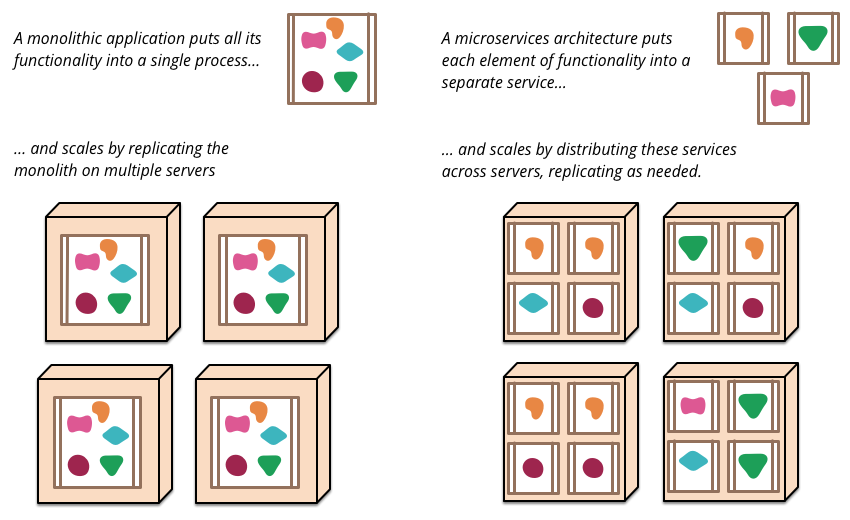
\includegraphics[width=\textwidth, center]{kapitel1/monolith_vs_microservices}
		\caption[Beschreibung für Verzeichnis]{Bildunterschrift}
		\label{img:microprofile}
	\end{figure}
	
	\subsection{Was sind Microservices}
	Lorem ipsum dolor sit amet, consetetur sadipscing elitr, sed diam nonumy eirmod tempor invidunt ut labore et dolore magna aliquyam erat, sed diam voluptua. At vero eos et accusam et justo duo dolores et ea rebum. Stet clita kasd gubergren, no sea takimata sanctus est Lorem ipsum dolor sit amet. Lorem ipsum dolor sit amet, consetetur sadipscing elitr, sed diam nonumy eirmod tempor invidunt ut labore et dolore magna aliquyam erat, sed diam voluptua. At vero eos et accusam et justo duo dolores et ea rebum. Stet clita kasd gubergren, no sea takimata sanctus est Lorem ipsum dolor sit amet \cite{Reese2009}.
	
	\paragraph{Klein und spezialisiert} Lorem ipsum dolor sit amet, consetetur sadipscing elitr, sed diam nonumy eirmod tempor invidunt ut labore et dolore magna aliquyam erat, sed diam voluptua. At vero eos et accusam et justo duo dolores et ea rebum. Stet clita kasd gubergren, no sea takimata sanctus est Lorem ipsum dolor sit amet. Lorem ipsum dolor sit amet, consetetur sadipscing elitr, sed diam nonumy eirmod tempor invidunt ut labore et dolore magna aliquyam erat, sed diam voluptua. At vero eos et accusam et justo duo dolores et ea rebum. Stet clita kasd gubergren, no sea takimata sanctus est Lorem ipsum dolor sit amet.
	
	\paragraph{Eigenständig} Lorem ipsum dolor sit amet, consetetur sadipscing elitr, sed diam nonumy eirmod tempor invidunt ut labore et dolore magna aliquyam erat, sed diam voluptua. At vero eos et accusam et justo duo dolores et ea rebum. Stet clita kasd gubergren, no sea takimata sanctus est Lorem ipsum dolor sit amet. Lorem ipsum dolor sit amet, consetetur sadipscing elitr, sed diam nonumy eirmod tempor invidunt ut labore et dolore magna aliquyam erat, sed diam voluptua. At vero eos et accusam et justo duo dolores et ea rebum. Stet clita kasd gubergren, no sea takimata sanctus est Lorem ipsum dolor sit amet. Verweis auf Anhang \ref{appendix:anhanga} \nameref{appendix:anhanga}
